The roubstness of the designed control design is verified by simulating three cases of off-nominal conditions. The parameters which vary are the inertia matrix, the residual magnetic dipole of the spacecraft and the initial conditions for the angular velocity and attitude quaternion. These simulated properties are reported in \cref{tab:off-nominal}.

\begin{table}[h!]
    \centering
    \caption{Properties for simulation of off-nominal conditions}
    \begin{tabular}{cccc}
    \toprule
    \toprule
    & \textbf{Case 1} & \textbf{Case 2} & \textbf{Case 3} \\
    \midrule
    $I \; [kg \cdot dm^2]$ & $\begin{bmatrix} 6.01 & -0.78 & 0.90 \\
    -0.78 & 7.71 & 0.05 \\
    0.90 & 0.05 & 9.81
    \end{bmatrix}$ & $\begin{bmatrix} 5.04 & 1.00 & -0.60 \\
    1.00 & 6.50 & 0.40 \\
    -0.60 & 0.40 & 8.41
    \end{bmatrix}$ & $\begin{bmatrix} 4.60 & -0.50 & -1.20 \\
    -0.50 & 8.31 & 1.10 \\
    -1.20 & 1.10 & 5.7
    \end{bmatrix}$\\
    \midrule
    $\mathbf{D}_r \; [A/m^2]$ & $ \begin{bmatrix} 0.02 & 0.04 & -0.10
    \end{bmatrix}$ & $ \begin{bmatrix} -0.04 & 0.05 & 0.10
    \end{bmatrix}$ & $ \begin{bmatrix} 0.08 & -0.05 & 0.04
    \end{bmatrix}$ \\
    \midrule
    $\bm{\omega}_0 \; [{}^{\circ}/s]$ & $\begin{bmatrix} 1 & 2 & 5
    \end{bmatrix}$ & $\begin{bmatrix} 4 & 10 & 9
    \end{bmatrix}$ & $\begin{bmatrix} 7 & 2 & 6
    \end{bmatrix}$\\
    \midrule
    $q_0 \; [-]$ & $\begin{bmatrix} 0.32 & 0.64 & 0.13 & 0.68
    \end{bmatrix}$ & $\begin{bmatrix} 0.55 & 0.30 & 0.75 & 0.19
    \end{bmatrix}$ & $\begin{bmatrix} 0.71 & 0.11 & 0.31 & 0.62
    \end{bmatrix}$ \\
    \bottomrule
    \bottomrule
    \end{tabular}
    \label{tab:off-nominal}
\end{table}

The cases are simulated only in the detumbling phase (with the proportional control) and in the tracking phase. The starting time of the simulations is set to $t = 0 \, s$ and each control phase lasts three orbital periods (as in the nominal case). The results of the analysis is reported through two of the most significant parameters ($\| \bm{\omega} \|$ for the detumbling phase and the pointing error in the tracking phase) in \cref{fig:offNominal-w,fig:offNominal-pe}.

\begin{figure}[h!]
    \centering
    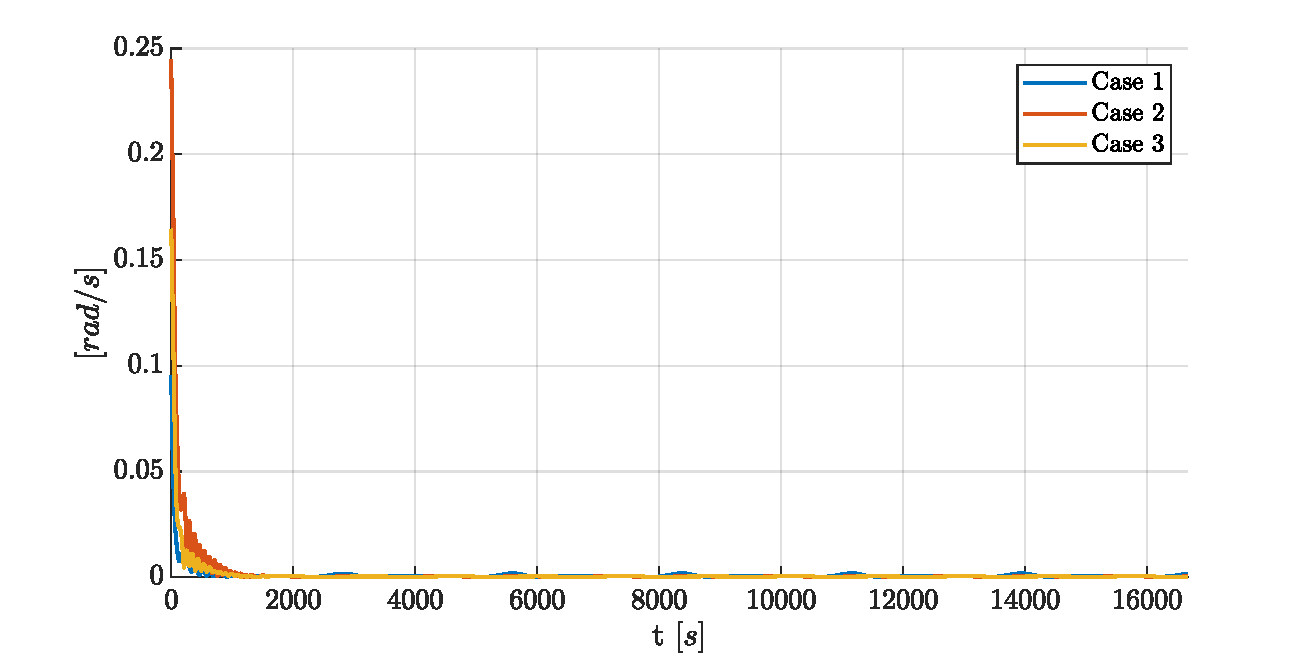
\includegraphics[width=0.8\textwidth]{graphics/offNominal/offNominal-w.pdf}
    \caption{Evolution of $\| \bm{\omega} \|$ (detumbling phase) in the off-nominal cases}
    \label{fig:offNominal-w}
\end{figure}

\begin{figure}[h!]
    \centering
    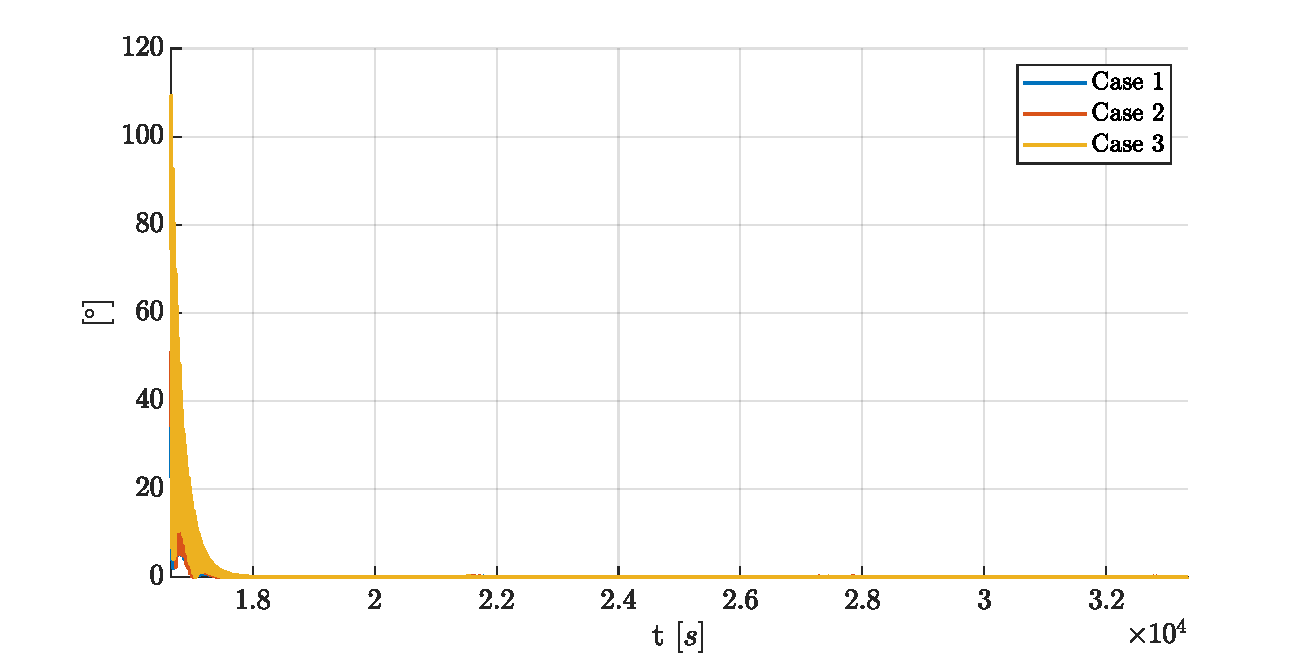
\includegraphics[width=0.8\textwidth]{graphics/offNominal/offNominal-pe.pdf}
    \caption{Evolution of the pointing error (tracking phase) in the off-nominal cases}
    \label{fig:offNominal-pe}
\end{figure}

It is clear that also in these cases the control system satisfies the requirements: the norm of the angular velocity drops to values below $10^{-3} \, rad/s$ in the detumbling phase, while the pointing error is in the order of $10^{-1 \; \circ}$ at the end of the tracking phase. The mission requirements for tracking are therefore still satisfied.

It is important to point out that the expression of the gravity gradient torque used throughout the simulations (\cref{eq:gravity-gradient}) is valid only in the principal axes of inertia, therefore only for diagonal matrices. The presence of the inertia products in the off-nominal conditions is neglected, so the same formula for $\mathbf{M}_{GG}$ is still applied. On the other hand, the disturbances introduced on the control system by the extra-diagonal terms of $I$ (as the control laws are designed on the nominal inertia matrix of the spacecraft) are counteracted through the disturbing torque estimated by the ESO \cite{biggs}.